\documentclass[a4paper,10pt]{article}
\usepackage[utf8]{inputenc}

\usepackage{graphicx}

%opening
\title{Task 2: baselines}
\author{Matthias}


\begin{document}

\maketitle

\section{Models}

I compare the following baselines in a 3 fold crossvalidation:
\begin{itemize}
 \item a linear regression model
 \item an autosklearn ensemble regressor, trained for 60 seconds per fold
\end{itemize}

Both models are trained and evaluated on the raw data and preprocessed (= standardized) data.
In both cases, only the configurations are used as input, not the time series (since this is task 2).


\section{Expectation}

I expect the autosklearn model to be (potentially much) better than the linear regression model,
since it's more powerful.

Extending the training time for the autosklearn model might improve the performance (this is not tested yet).

The preprocessing might improve both models' performance a little bit.


\section{Results}

Predicted y over true y for the linear regression model without preprocessing:

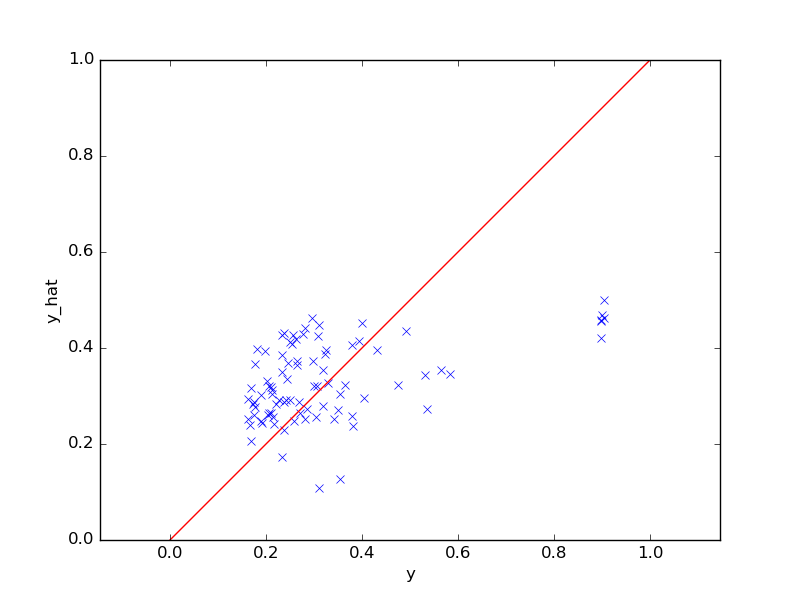
\includegraphics[width=0.8\textwidth]{../../figures/baseline_LinearRegression_predictions}

Predicted y over true y for the linear regression model with preprocessing:

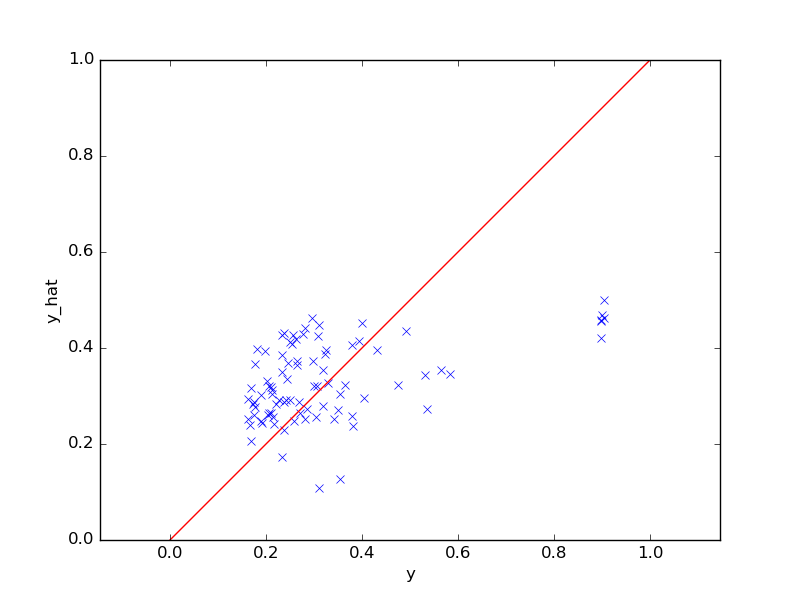
\includegraphics[width=0.8\textwidth]{../../figures/baseline_LinearRegression_standardized_predictions} \\
(side note: is linear regression invariant to scaling and shifting? $\rightarrow$ that would explain why the results are the same)

\vspace{0.5cm}
Predicted y over true y for the autosklearn ensemble without preprocessing:

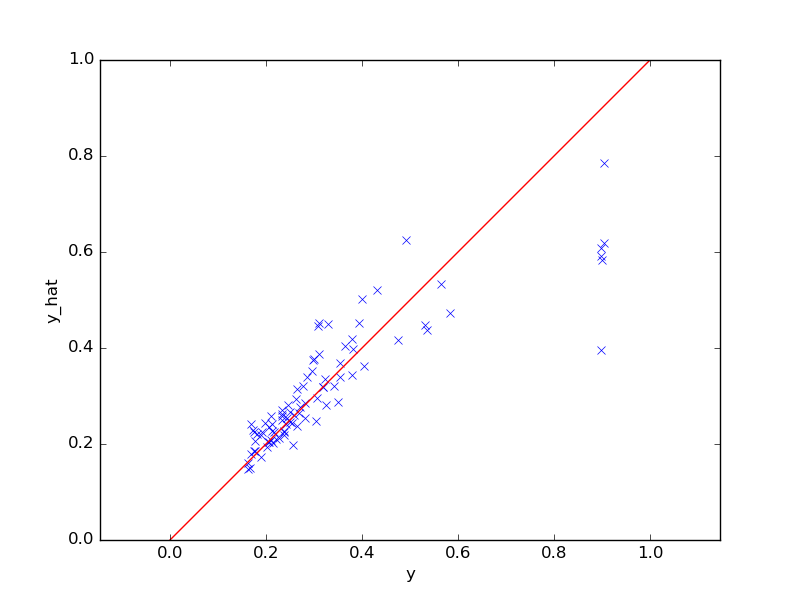
\includegraphics[width=0.8\textwidth]{../../figures/baseline_autosklearn_60s_predictions}

Predicted y over true y for the autosklearn ensemble with preprocessing:

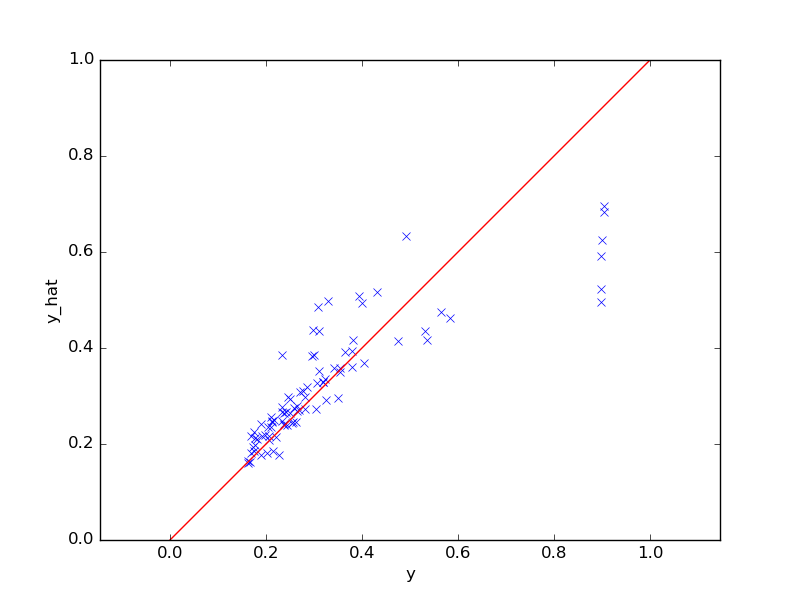
\includegraphics[width=0.8\textwidth]{../../figures/baseline_autosklearn_60s_standardized_predictions}

Mean CV loss (mean squared error):

\vspace{0.5cm}
\begin{tabular}{|c|c|c|}
 \hline
 model & raw & standardized \\
 \hline
 linear regression & 0.032744 & 0.032744 \\
 autosklearn & 0.012119 & 0.010339 \\
 \hline
\end{tabular}

\vspace{0.5cm}
Keep in mind that autosklearn is randomized.
I once got a mean CV loss below 0.01 for autosklearn without preprocessing.
We should probably fix the random seed.\\
Most likely autosklearn does preprocessing internally.


\section{Conclusions}

\begin{itemize}
 \item preprocessing has no effect on linear regression and autosklearn
 \item predicting the cases with y $>$ 0.8 might be hard (it is hard for autosklearn)
 \item we would like to achieve a mean squared error below 0.01 to beat the baselines
\end{itemize}


\end{document}
